
\lhead[\chaptername~\thechapter]{\rightmark}


\rhead[\leftmark]{}


\lfoot[\thepage]{}


\cfoot{}


\rfoot[]{\thepage}


\chapter{The Game}


\section{Your first game}

When you first launch \mbox{Super Hangman}, you will be presented
with a game screen similar to that in \ref{fig:Initial-load-screen}.
This screen has two main parts which display various aspects of the
current game session.

\begin{figure}[h]
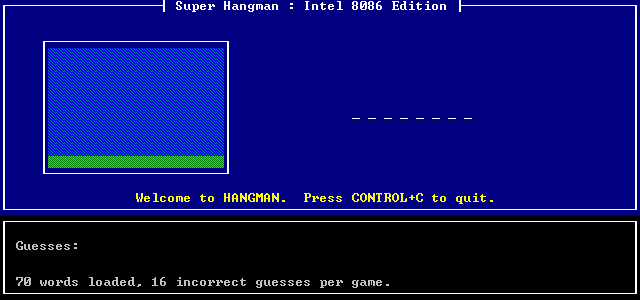
\includegraphics[scale=0.5]{new_game}

\caption{\label{fig:Initial-load-screen}Initial load screen}
\end{figure}


The first part, the black portion, displays the letters you have currently
guessed, the number of incorrect guesses you have left before the
game ends, and information about the current game (such as the number
of words the game can choose from).

The second part, the blue portion, displays the word you must guess,
information on your current guess, and a traditional Hangman-like
pictorial.

Once this screen has loaded, you are ready to make your first guess.


\section{Making your first guess}

Simply press any alphabetic key on your keyboard to start making a
guess. You do not need worry about pressing the \texttt{SHIFT} or
\texttt{CAPS LOCK} keys, as all words and guesses will automatically
be treated as capital letters. Any non-alphabetic keys will be ignored
without being treated as an incorrect guess.

Once you have made your guess you will be told if your guess is correct
or incorrect. If your guess completes a word, the game will end at
this point and you will be informed of your success. Likewise, if
your guess results in your last ``life'' being used, you will be
informed of your loss. With both winning and losing, you will be asked
if you want to start a new game. Simply press \texttt{Y} for a new
game, or N to exit \mbox{Super Hangman}.


\section{The results of guessing}

As we saw in the previous section, one of a few things will happen
after you make a guess and there will be several changes to the screen.
Let us look at some of these changes.


\subsection{Correct guesses}

\begin{figure}[h]
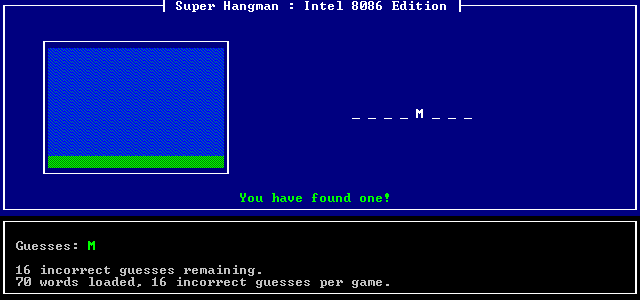
\includegraphics[scale=0.5]{correct_guess}

\caption{\label{fig:A-correct-guess}A correct guess}
\end{figure}


When you make a correct guess, the guessed letter will be added to
the ``Guesses'' section in green text. This is to remind you that
you have previously guessed this letter, and that it was a correct
guess. The word in the right-hand side of the blue section will also
display each letter in the word that you have guessed. Once you guess
a correct letter and should the word contain more than one of that
letter, they will be all displayed for you. You do not have to guess
that letter more than once. The game will also inform you that you
have made a correct guess. The screen for a correct guess will look
similar to \ref{fig:A-correct-guess}.


\subsection{Incorrect guesses}

\begin{figure}[h]
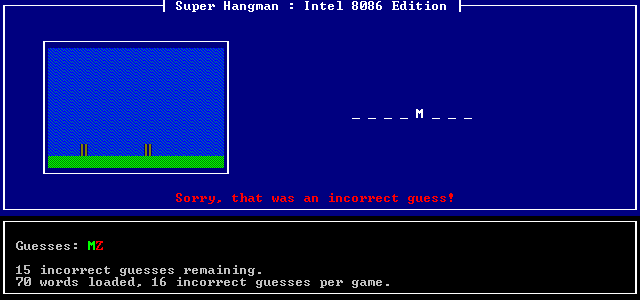
\includegraphics[scale=0.5]{incorrect_guess}

\caption{\label{fig:An-incorrect-guess}An incorrect guess}


\end{figure}


When you make an incorrect guess, the guessed letter will be added
to the ``Guesses'' section in red text. This is to remind you that
you have previously guessed this letter, and that it was an incorrect
guess. The game will also inform you that you have made an incorrect
guess. The screen for an incorrect guess will look similar to \ref{fig:An-incorrect-guess}.


\subsection{Repeated guesses}

\begin{figure}[h]
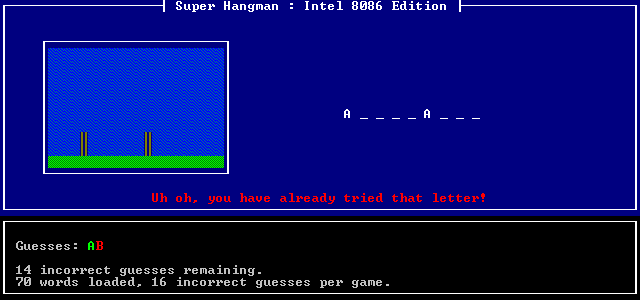
\includegraphics[scale=0.5]{repeat_guess}

\caption{\label{fig:A-repeat-guess}A repeat guess}


\end{figure}


When you repeat a previous guess, the game will simply inform you
that you have repeated a guess without adding anything to the ``Guesses''
section. The number of incorrect guesses that you have left will go
down by one and the stick figure will be one step closer to oblivion.
Should you repeat a guess, the screen will look similar to \ref{fig:A-repeat-guess}.


\subsection{Winning a game}

\begin{figure}[h]
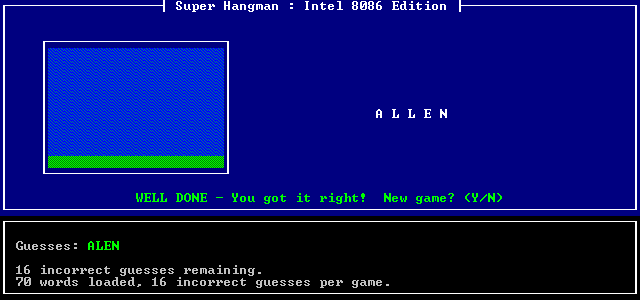
\includegraphics[scale=0.5]{game_won}

\caption{\label{fig:Winning-a-game}Winning a game}


\end{figure}

